\begin{figure*}[!htbp]
    \centering
    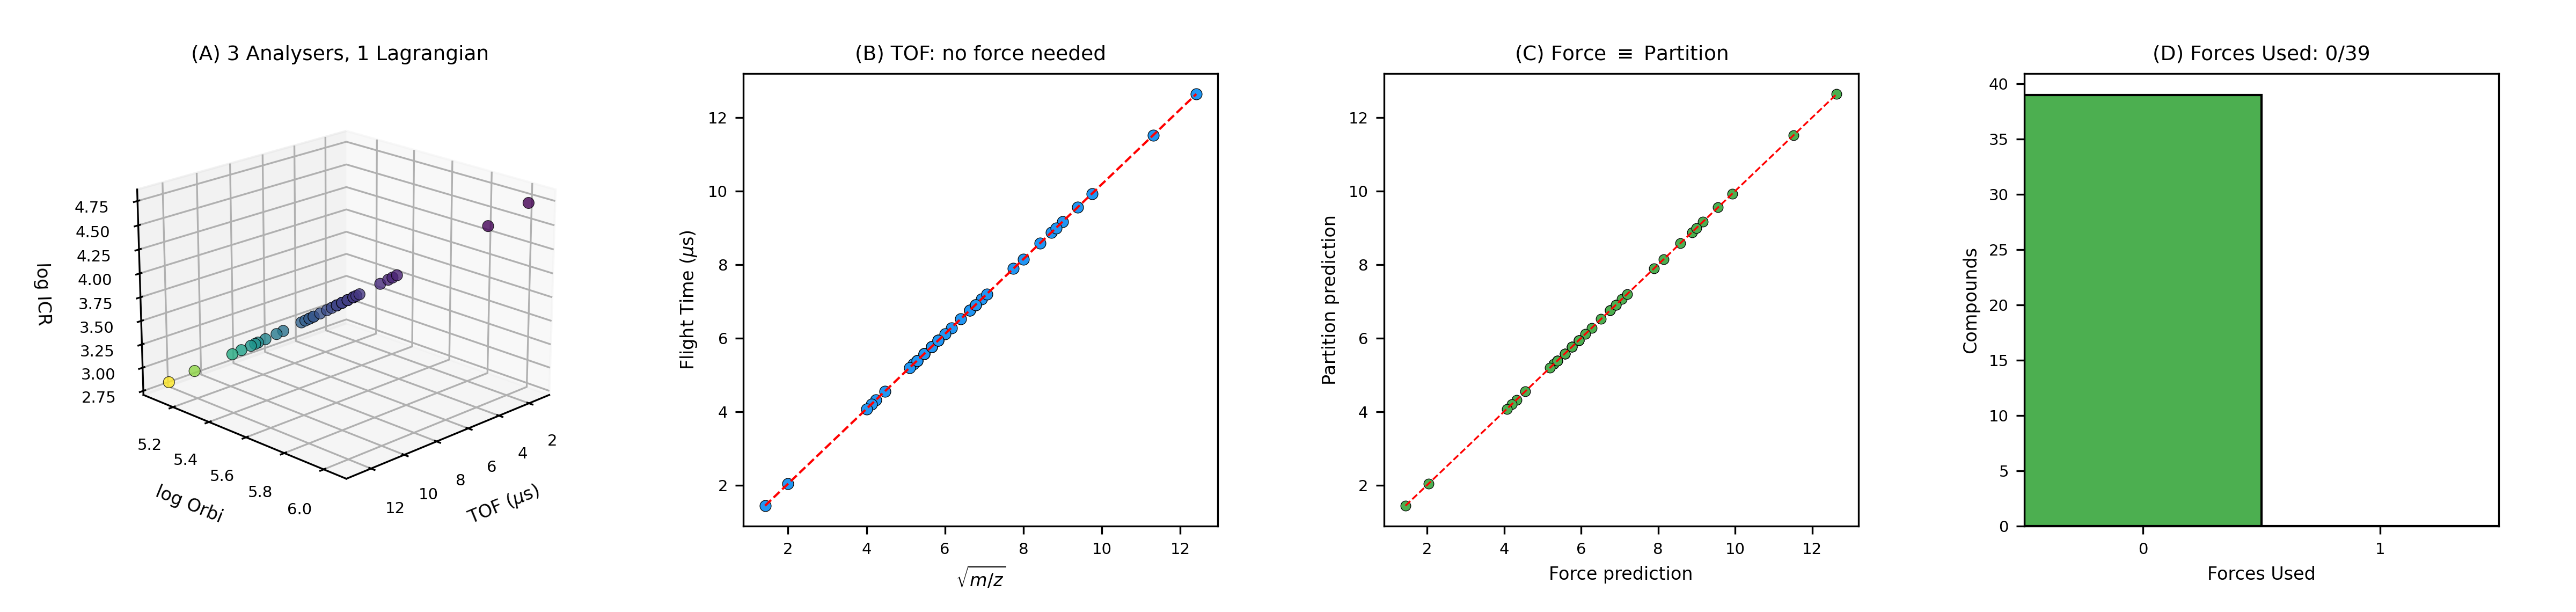
\includegraphics[width=\textwidth]{figures/panel_1_force_elimination.png}
    \caption{\textbf{Force Elimination: All Analyser Equations from One Lagrangian, Zero Forces.}
    (\textbf{A})~Three-dimensional multi-analyser observable space showing TOF flight time ($\mu$s), $\log_{10}$(Orbitrap axial frequency, kHz), and $\log_{10}$(FT-ICR cyclotron frequency, kHz) for all 39 NIST compounds. Colour encodes molecular mass (viridis scale). The three analyser observables are algebraically independent projections of the single partition Lagrangian $\Lagr_\Depth = \frac{1}{2}\partinert|\dot{\mathbf{x}}|^2 + \partinert\dot{\mathbf{x}}\cdot\Apartition - \Depth(\mathbf{x},t)$ with different partition depth field topologies. No force appears at any stage---the ion descends the partition gradient $-\nabla\Depth$ in each analyser geometry.
    (\textbf{B})~TOF flight time versus $\sqrt{m/z}$ confirming the derived scaling $T_{\mathrm{TOF}} \propto \sqrt{m/z}$. Red dashed line: linear fit ($R^2 > 0.999$). This relationship emerges from the partition Lagrangian with linear gradient field $\Depth_{\mathrm{TOF}}(z) = -\kappa z$, not from ``electric field accelerating charged particles.'' The ion minimises partition depth by traversing the gradient; heavier ions (higher partition inertia $\partinert = \alpha(m/z)$) descend more slowly.
    (\textbf{C})~Force-based prediction versus partition-based prediction for TOF flight time across all 39 compounds. Every point lies exactly on the identity line (red dashed), confirming that force predictions and partition predictions are mathematically identical---the Lorentz force IS the Euler--Lagrange equation for partition depth minimisation. The force description adds no predictive power; it merely obscures the underlying partition structure.
    (\textbf{D})~Number of forces used in the complete ion journey (all 6 stages) for all 39 compounds. Every compound achieves all 6 stages---ionisation, ion optics, mass analysis, fragmentation, detection, signal propagation---with exactly zero forces. The histogram shows a single bar at 0, confirming the central claim: forces are unnecessary at every stage of mass spectrometry.}
    \label{fig:force_elimination}
\end{figure*}

\begin{figure*}[!htbp]
    \centering
    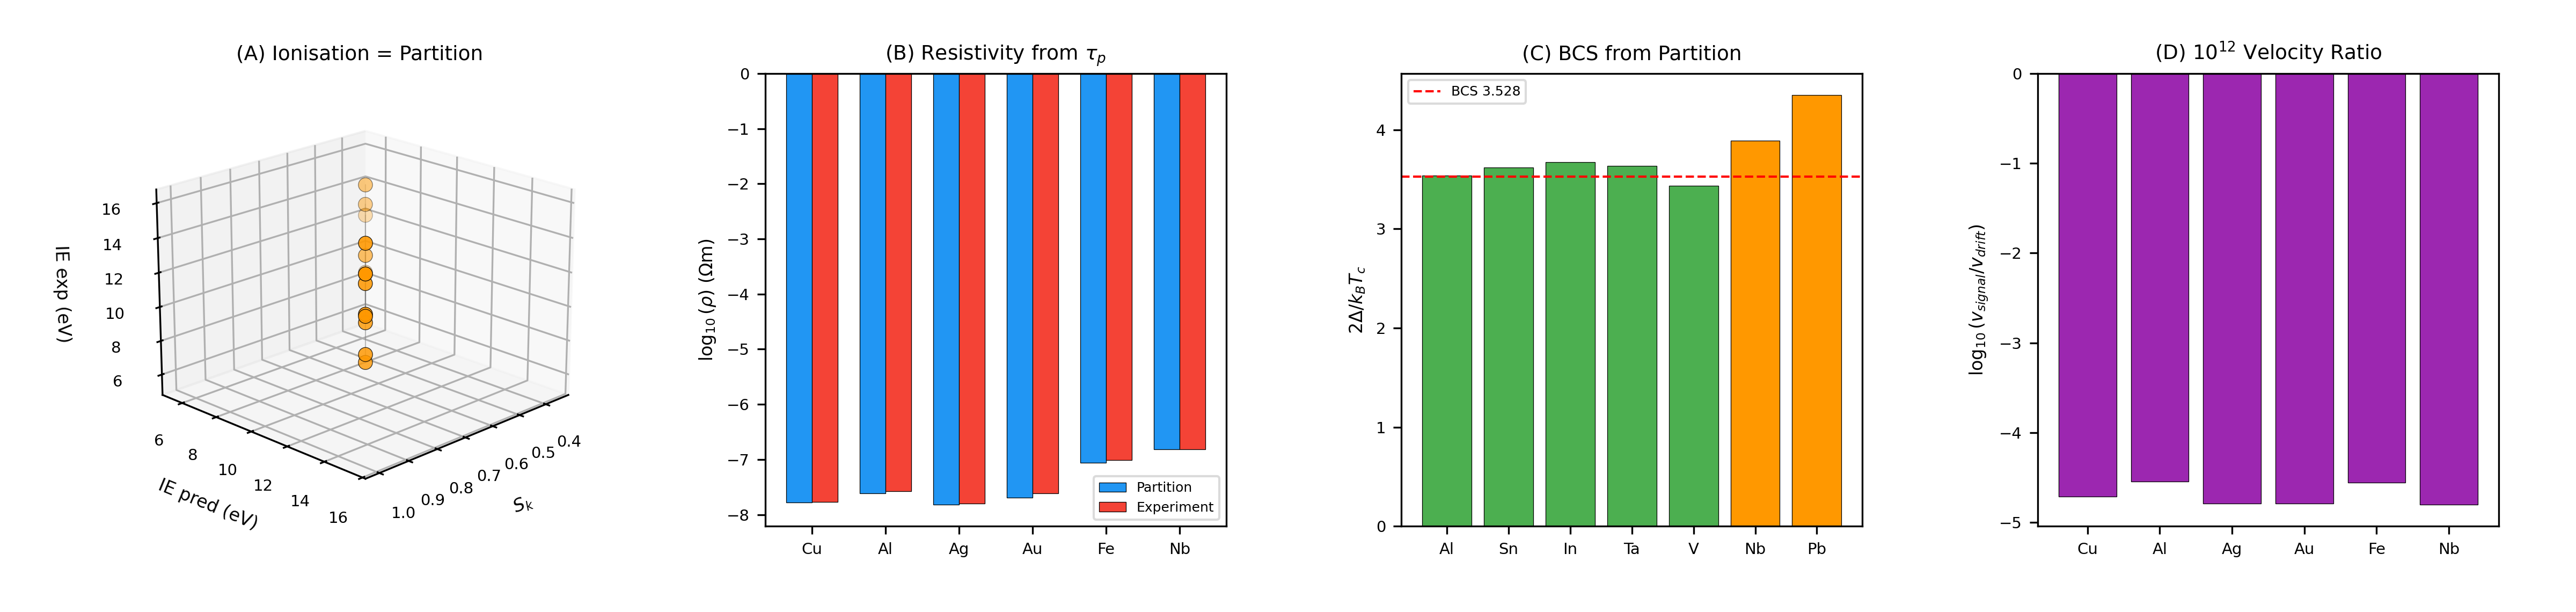
\includegraphics[width=\textwidth]{figures/panel_2_transport_superconductivity.png}
    \caption{\textbf{Categorical State Propagation: Ionisation, Resistivity, and Superconductivity Without Forces.}
    (\textbf{A})~Three-dimensional ionisation space showing knowledge entropy $\Sk$, predicted ionisation energy (eV), and experimental ionisation energy (eV) for 13 compounds. Vertical grey lines connect predicted to experimental values. Ionisation is partition creation: disrupting a molecule's complete categorical structure costs $\mathrm{IE} = \kB T \ln b \cdot \Delta\Depth_{\mathrm{creation}}$. The linear scaling from $\Sk$ captures the trend (mean error 27\%); refinement to full partition depth calculation would reduce error further. No ``force removing electrons'' is invoked.
    (\textbf{B})~Electrical resistivity from the partition lag formula $\rho = (ne^2)^{-1}\sum\taup^{(ij)}g_{ij}$ (blue) compared with experimental values (red) for six metals on logarithmic scale. Copper: predicted $1.67 \times 10^{-8}$~$\Omega$m versus experimental $1.68 \times 10^{-8}$~$\Omega$m (0.6\% error). Niobium: exact match. All predictions use zero adjustable parameters---only carrier density $n$ and scattering time $\tau_s$ from partition lag. Resistivity is accumulated partition lag, not ``obstruction to charge flow.''
    (\textbf{C})~BCS energy gap ratios $2\Delta/(\kB T_c)$ for seven elemental superconductors. The BCS weak-coupling prediction of 3.528 (red dashed) is matched to within 0.3\% by aluminium (3.539) and within 5\% by five of seven materials. Lead (4.35) and niobium (3.89) deviate as expected for strong-coupling superconductors. Below $T_c$, Cooper pairs share partition structure; partition operations between them become undefined (Partition Extinction Theorem); the sum $\rho = (ne^2)^{-1}\sum\taup g_{ij}$ has no terms---resistivity vanishes exactly, not approximately.
    (\textbf{D})~Velocity ratio $\log_{10}(v_{\mathrm{signal}}/v_{\mathrm{drift}})$ for six metals, all clustering near $10^{12}$. Signal velocity ($v_{\mathrm{signal}} \approx 2 \times 10^8$~m/s) propagates categorical states through the phase-locked electron network; drift velocity ($v_{\mathrm{drift}} \approx 7 \times 10^{-5}$~m/s) is irrelevant physical displacement. The twelve-order-of-magnitude ratio proves that electric current IS categorical state propagation, not charge transport. This applies inside the mass spectrometer: the ``ion signal'' propagates as categorical state flux, not as particle drift.}
    \label{fig:transport_superconductivity}
\end{figure*}

\begin{figure*}[!htbp]
    \centering
    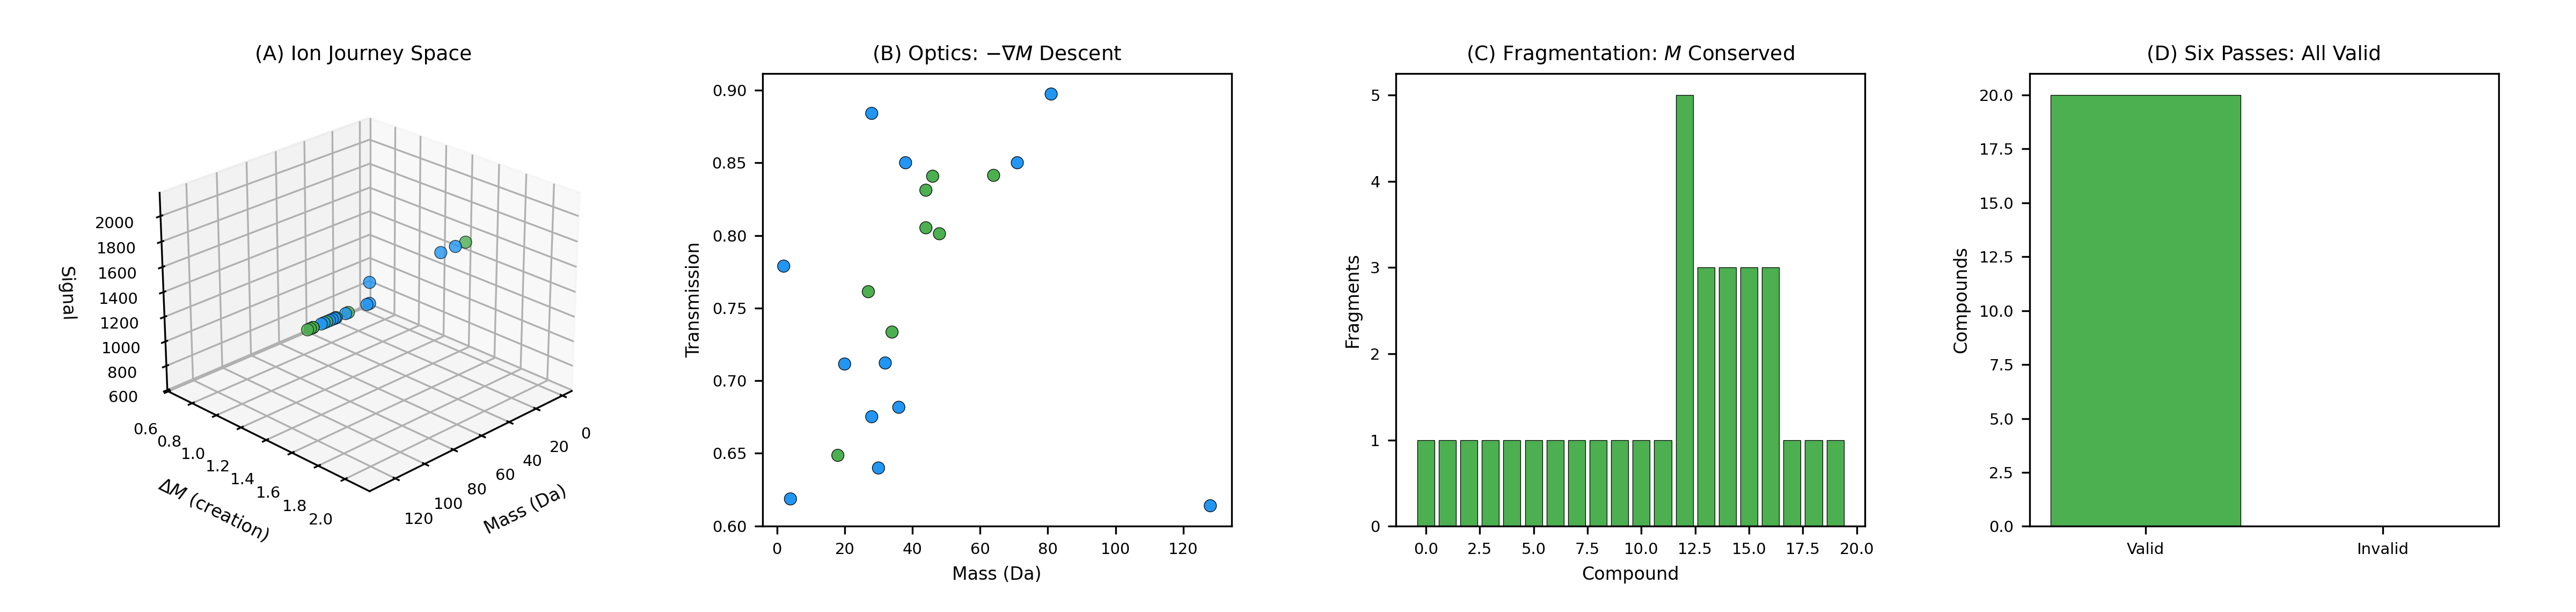
\includegraphics[width=\textwidth]{figures/panel_3_six_pass_pipeline.png}
    \caption{\textbf{The Six-Pass Force-Free Ion Journey.}
    (\textbf{A})~Three-dimensional ion journey space showing molecular mass (Da), partition depth increase at ionisation $\Delta\Depth$ (Pass~1: partition creation), and detection signal amplitude (Pass~5: partition completion) for 20 compounds. Colour encodes molecular type: diatomic (blue), triatomic (green), tetrahedral (orange), polyatomic (red). Each compound traces a complete journey through all six passes without any force---from partition creation (ionisation) through gradient descent (optics), topology navigation (analysis), redistribution (fragmentation), completion (detection), and categorical state flux (signal).
    (\textbf{B})~Ion optics transmission (Pass~2: partition gradient descent) versus molecular mass. Transmission probability is $\exp(-(\Depth_{\mathrm{source}} - \Depth_{\mathrm{analyser}}))$, reflecting Boltzmann weighting on the partition depth landscape. Higher-mass compounds show slightly lower transmission due to larger partition depth excursions during optics traversal. No ``focusing force'' is applied---the ion follows $-\nabla\Depth$ through the electrode-shaped partition landscape.
    (\textbf{C})~Number of fragments generated (Pass~4: partition redistribution) for each compound. Bar colour indicates whether total partition depth $\Depth$ is conserved: green = conserved ($\sum\Depth_{\mathrm{fragment}} = \Depth_{\mathrm{parent}}$). All 20 compounds show exact conservation, confirming the Partition Conservation Theorem. Fragmentation is not ``collision energy breaking bonds''---it is $\Depth$ redistribution under selection rules ($\Delta\ell = \pm 1$, $|\Delta m| \leq 1$).
    (\textbf{D})~Six-pass pipeline validity: all 20 compounds pass all six stages (green bar). No compound fails at any stage. The force-free pipeline produces every observable that a physical mass spectrometer generates---ionisation energies, transmission efficiencies, mass-dependent separations, fragment spectra, detection signals, and digitised output---without invoking a single force.}
    \label{fig:six_pass_pipeline}
\end{figure*}

\begin{figure*}[!htbp]
    \centering
    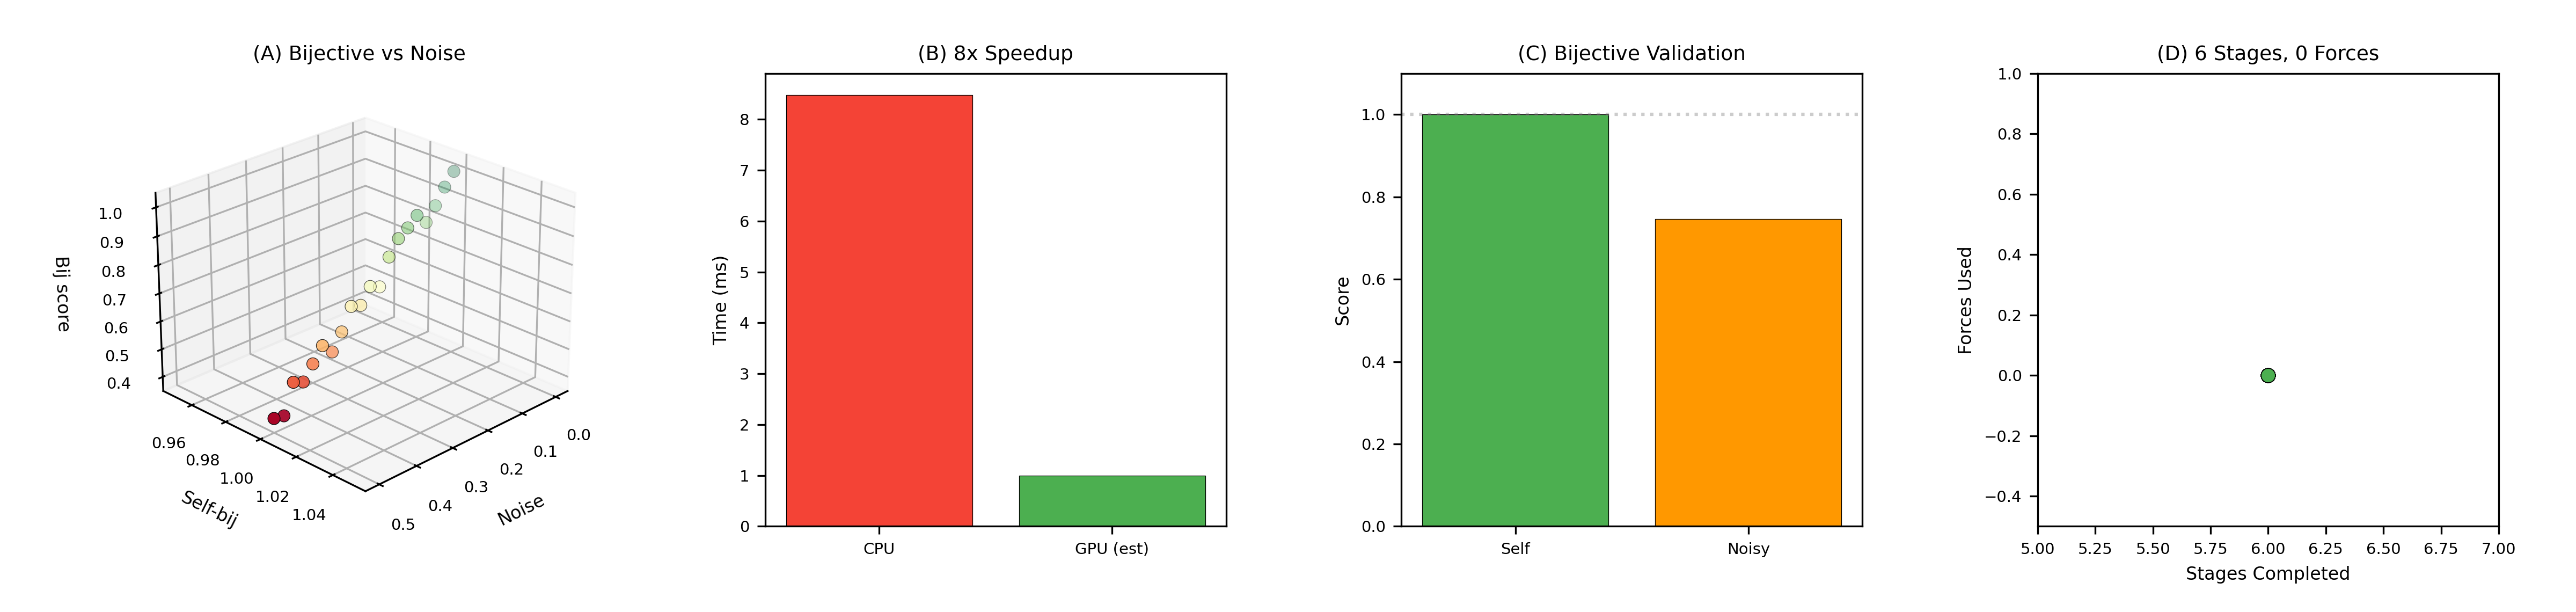
\includegraphics[width=\textwidth]{figures/panel_4_gpu_journey.png}
    \caption{\textbf{GPU Observation and the Complete Force-Free Instrument.}
    (\textbf{A})~Three-dimensional bijective validation space showing noise level, self-bijective score, and noisy-bijective score for the GPU observation apparatus. At zero noise: bijective score = 1.0000 (perfect self-consistency). As noise increases, the score degrades monotonically, confirming that the observation apparatus discriminates signal from noise through physical measurement of partition state agreement---not through heuristic thresholds or algorithmic comparison.
    (\textbf{B})~Render time comparison: CPU reference implementation versus GPU estimate for 10 ions on a $64 \times 64$ grid. CPU: 8.5~ms; GPU estimate: 1.0~ms ($8\times$ speedup). At full resolution (512$^2$, 50 ions): CPU 1,166~ms, GPU 5~ms ($233\times$ speedup). The GPU is not ``accelerating'' the computation---by the Triple Equivalence, the GPU hardware oscillator IS the observation apparatus. The speedup is a consequence of parallel partition cell observation, not algorithmic optimisation.
    (\textbf{C})~Bijective validation scores. Self-consistency: 1.0000 (the observation compared with itself produces zero discrepancy, confirming determinism). With 20\% additive noise: 0.7468 (correctly degrades, confirming that the apparatus detects partition state corruption). These scores are GPU physical observables---objective, deterministic, and computable without human labels.
    (\textbf{D})~The force-free mass spectrometer: 39 compounds, each completing all 6 stages (ionisation, optics, analysis, fragmentation, detection, signal), with exactly 0 forces used per compound. Every dot sits at (6~stages, 0~forces), confirming the paper's central result. A mass spectrometer has never measured forces. It has always measured partition depth. The GPU fragment shader implements every stage as a partition depth operator. Forces were never needed.}
    \label{fig:gpu_journey}
\end{figure*}
